\documentclass[12pt, twoside]{article}
\usepackage{amsmath}
\usepackage{amssymb}
\usepackage{graphicx}
\usepackage{enumerate}
\usepackage{geometry}
\usepackage{pgfplots}
\pgfplotsset{compat=1.18}
\usepackage{tikz}
\geometry{margin=1in}

\begin{document}

\begin{center}
\Large{\textbf{IB Mathematics: Analysis and Approaches}} \\
\large{\textbf{Standard Level -- Paper 1}} \\
\normalsize{8 May 2023 -- No Calculator} \\
\normalsize{80 marks total}
\end{center}

\vspace{0.5cm}

\section*{Section A}

\begin{enumerate}

% Question 1 [5 marks]
\item \textbf{[5 marks]} Point P has coordinates $(-3, 2)$, and point Q has coordinates $(15, -8)$. Point M is the midpoint of [PQ].
    \begin{enumerate}[(a)]
        \item Find the coordinates of M.
    \end{enumerate}
    Line $L$ is perpendicular to [PQ] and passes through M.
    \begin{enumerate}[(a)]
        \setcounter{enumii}{1}
        \item Find the gradient of $L$.
        \item Hence, write down the equation of $L$.
    \end{enumerate}

\vspace{1cm}

% Question 2 [7 marks]
\item \textbf{[7 marks]} The function $f$ is defined by $f(x) = \frac{7x+7}{2x-4}$ for $x \in \mathbb{R}$, $x \neq 2$.
    \begin{enumerate}[(a)]
        \item Find the zero of $f(x)$.
        \item For the graph of $y = f(x)$, write down the equation of
        \begin{enumerate}[(i)]
            \item the vertical asymptote;
            \item the horizontal asymptote.
        \end{enumerate}
        \item Find $f^{-1}(x)$, the inverse function of $f(x)$.
    \end{enumerate}

\vspace{1cm}

% Question 3 [6 marks]
\item \textbf{[6 marks]} On a Monday at an amusement park, a sample of 40 visitors was randomly selected as they were leaving the park. They were asked how many times that day they had been on a ride called \textit{The Dragon}. This information is summarized in the following frequency table.

\begin{center}
\begin{tabular}{|c|c|}
\hline
\textbf{Number of times on \textit{The Dragon}} & \textbf{Frequency} \\
\hline
0 & 6 \\
1 & 16 \\
2 & 13 \\
3 & 2 \\
4 & 3 \\
\hline
\end{tabular}
\end{center}

It can be assumed that this sample is representative of all visitors to the park for the following day.

    \begin{enumerate}[(a)]
        \item For the following day, Tuesday, estimate
        \begin{enumerate}[(i)]
            \item the probability that a randomly selected visitor will ride \textit{The Dragon};
            \item the expected number of times a visitor will ride \textit{The Dragon}.
        \end{enumerate}
    \end{enumerate}
    
    It is known that 1000 visitors will attend the amusement park on Tuesday. \textit{The Dragon} can carry a maximum of 10 people each time it runs.
    
    \begin{enumerate}[(a)]
        \setcounter{enumii}{1}
        \item Estimate the minimum number of times \textit{The Dragon} must run to satisfy demand.
    \end{enumerate}

\vspace{1cm}

% Question 4 [6 marks]
\item \textbf{[6 marks]}
    \begin{enumerate}[(a)]
        \item Show that the equation $\cos 2x = \sin x$ can be written in the form $2\sin^2 x + \sin x - 1 = 0$.
        \item Hence, solve $\cos 2x = \sin x$, where $-\pi \leq x \leq \pi$.
    \end{enumerate}

\vspace{1cm}

% Question 5 [6 marks]
\item \textbf{[6 marks]} Find the range of possible values of $k$ such that $e^{2x} + \ln k = 3e^x$ has at least one real solution.

\vspace{1cm}

% Question 6 [6 marks]
\item \textbf{[6 marks]} The function $f$ is defined by $f(x) = \sin qx$, where $q > 0$. The following diagram shows part of the graph of $f$ for $0 \leq x \leq 4m$, where $x$ is in radians. There are $x$-intercepts at $x = 0$, $2m$ and $4m$.

\begin{center}
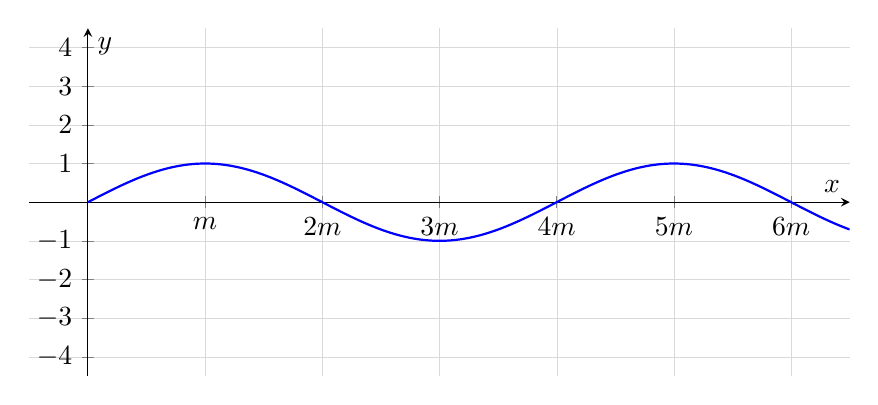
\begin{tikzpicture}
\begin{axis}[
    width=12cm,
    height=6cm,
    axis lines=middle,
    xlabel={$x$},
    ylabel={$y$},
    xmin=-0.5, xmax=6.5,
    ymin=-4.5, ymax=4.5,
    xtick={1,2,3,4,5,6},
    xticklabels={$m$,$2m$,$3m$,$4m$,$5m$,$6m$},
    ytick={-4,-3,-2,-1,0,1,2,3,4},
    grid=major,
    grid style={line width=.1pt, draw=gray!30},
    samples=200,
    smooth,
]
% f(x) = sin(pi*x/2) so that zeros are at x=0,2,4 (when x is in units of m)
\addplot[domain=0:6.5, blue, thick] {sin(deg(pi*x/2))};
\end{axis}
\end{tikzpicture}
\end{center}

    \begin{enumerate}[(a)]
        \item Find an expression for $m$ in terms of $q$.
    \end{enumerate}
    
    The function $g$ is defined by $g(x) = 3\sin\frac{2qx}{3}$, for $0 \leq x \leq 6m$.
    
    \begin{enumerate}[(a)]
        \setcounter{enumii}{1}
        \item On the axes above, sketch the graph of $g$.
    \end{enumerate}

\newpage

\section*{Section B}

\setcounter{enumi}{6}

% Question 7 [13 marks]
\item \textbf{[13 marks]} The function $h$ is defined by $h(x) = 2xe^x + 3$, for $x \in \mathbb{R}$. The following diagram shows part of the graph of $h$, which has a local minimum at point A.

\begin{center}
\begin{tikzpicture}
\begin{axis}[
    width=10cm,
    height=8cm,
    axis lines=middle,
    xlabel={$x$},
    ylabel={$y$},
    xmin=-3, xmax=2,
    ymin=-1, ymax=10,
    xtick={-3,-2,-1,0,1,2},
    ytick={0,2,4,6,8,10},
    samples=200,
    smooth,
]
\addplot[domain=-3:2, blue, thick] {2*x*exp(x) + 3};
\node[circle, fill=black, inner sep=2pt, label=above right:{A}] at (-1, 2.26) {};
\end{axis}
\end{tikzpicture}
\end{center}

    \begin{enumerate}[(a)]
        \item Find the value of the $y$-intercept.
        \item Find $h'(x)$.
        \item Hence, find the coordinates of A.
        \item \begin{enumerate}[(i)]
            \item Show that $h''(x) = (2x + 4)e^x$.
            \item Find the values of $x$ for which the graph of $h$ is concave-up.
        \end{enumerate}
    \end{enumerate}

\vspace{1cm}

% Question 8 [14 marks]
\item \textbf{[14 marks]} Consider the arithmetic sequence $u_1, u_2, u_3, \ldots$.

The sum of the first $n$ terms of this sequence is given by $S_n = n^2 + 4n$.

    \begin{enumerate}[(a)]
        \item \begin{enumerate}[(i)]
            \item Find the sum of the first five terms.
            \item Given that $S_6 = 60$, find $u_6$.
        \end{enumerate}
        \item Find $u_1$.
        \item Hence or otherwise, write an expression for $u_n$ in terms of $n$.
    \end{enumerate}
    
    Consider a geometric sequence, $v_n$, where $v_2 = u_1$ and $v_4 = u_6$.
    
    \begin{enumerate}[(a)]
        \setcounter{enumii}{3}
        \item Find the possible values of the common ratio, $r$.
        \item Given that $v_{99} < 0$, find $v_5$.
    \end{enumerate}

\vspace{1cm}

% Question 9 [17 marks]
\item \textbf{[17 marks]} An object moves along a straight line. Its velocity, $v\text{ ms}^{-1}$, at time $t$ seconds is given by
\[
v(t) = -t^3 + \frac{7}{2}t^2 - 2t + 6, \text{ for } 0 \leq t \leq 4.
\]
The object first comes to rest at $t = k$.

The graph of $v$ is shown in the following diagram.

\begin{center}
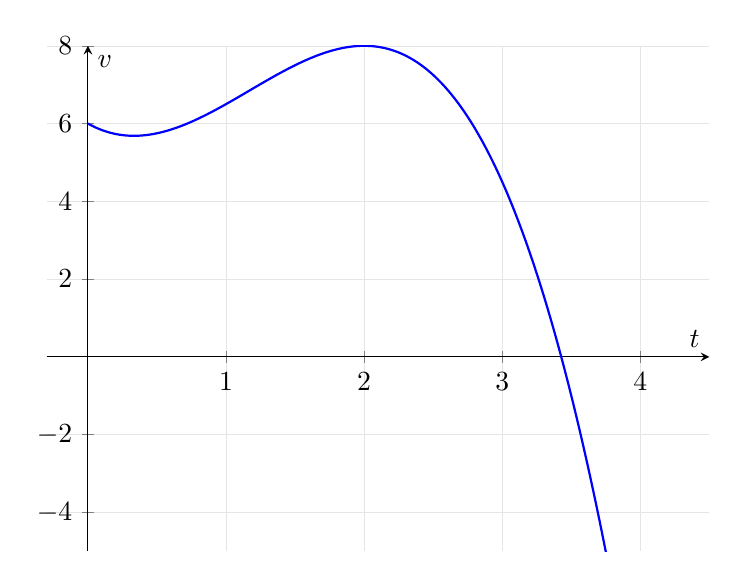
\begin{tikzpicture}
\begin{axis}[
    width=10cm,
    height=8cm,
    axis lines=middle,
    xlabel={$t$},
    ylabel={$v$},
    xmin=-0.3, xmax=4.5,
    ymin=-5, ymax=8,
    xtick={0,1,2,3,4},
    ytick={-4,-2,0,2,4,6,8},
    samples=200,
    smooth,
    grid=major,
    grid style={line width=.1pt, draw=gray!20},
]
\addplot[domain=0:4, blue, thick] {-x^3 + 3.5*x^2 - 2*x + 6};
\end{axis}
\end{tikzpicture}
\end{center}

At $t = 0$, the object is at the origin.

    \begin{enumerate}[(a)]
        \item Find the displacement of the object from the origin at $t = 1$.
        \item Find an expression for the acceleration of the object.
        \item Hence, find the greatest speed reached by the object before it comes to rest.
        \item Find the greatest speed reached by the object for $0 \leq t \leq 4$.
        \item Write down an expression that represents the distance travelled by the object while its speed is increasing. Do not evaluate the expression.
    \end{enumerate}

\end{enumerate}

\end{document}
